\section{\texorpdfstring{Phương pháp nghiên cứu}{methodology}}
% Trình bày chi tiết về ý tưởng, các mô hình toán, các chứng minh nếu có. Đồng thời trình bày các bước thực hiện và khảo sát, kiểm nghiệm kết quả nghiên cứu. Mô tả kết quả nghiên cứu khi thử nghiệm với nhiều tập dữ liệu và những độ khó khác nhau.

\subsection{Ý tưởng thực hiện luận văn}

Nhắc lại yêu cầu bài toán: Tạo sinh video khuôn mặt người đang nói dựa trên một hình ảnh tĩnh chứa mặt người mẫu và một đoạn âm thanh chứa tiếng nói.

Dựa theo yêu cầu bài toán, ta cần tìm kiếm một phương pháp để kết hợp đặc trưng âm thanh và hình ảnh lại với nhau, sau đó chuyển đổi đặc trưng này thành video.

\subsection{Mô hình hóa bài toán}

\subsection{Các tập dữ liệu được sử dụng}
\subsubsection{Tập dữ liệu GRID}
\subsubsection{Tập dữ liệu LRW}

\subsection{Tiền xử lý dữ liệu}

\subsection{Cấu trúc tổng quát của hệ thống}

\subsection{Cấu trúc của bộ giải mã landmark của khuôn mặt (Landmark Decoder)}

\begin{figure}[H]
    \centering
    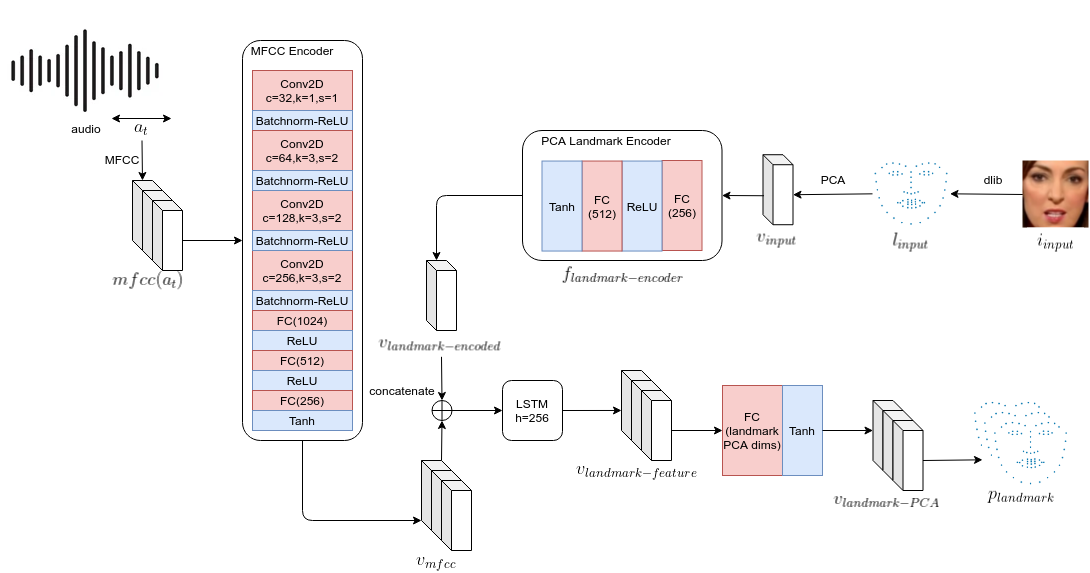
\includegraphics[width=15cm]{./content/materials/landmark_decoder.png}
    \caption{Cấu trúc của bộ giải mã landmark của khuôn mặt (Landmark Decoder)}
\end{figure}

\subsection{Cấu trúc của bộ tạo sinh hình ảnh (Generator)}

\begin{figure}[H]
    \centering
    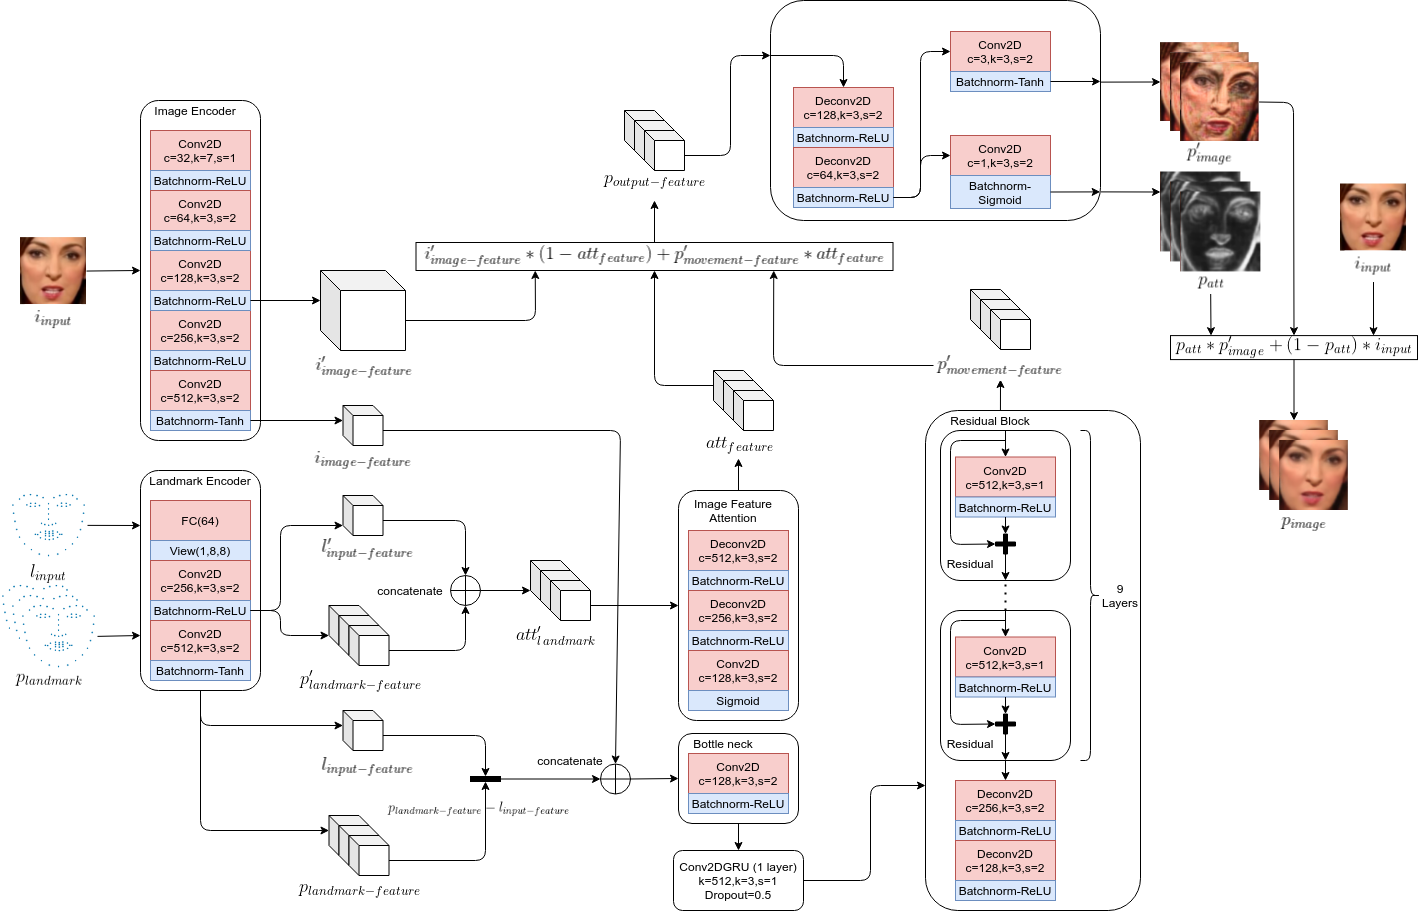
\includegraphics[width=15cm]{./content/materials/generator.png}
    \caption{Cấu trúc của bộ giải mã landmark của khuôn mặt (Generator)}
\end{figure}

\subsection{Cấu trúc của bộ phân biệt hình ảnh (Discriminator)}

\begin{figure}[H]
    \centering
    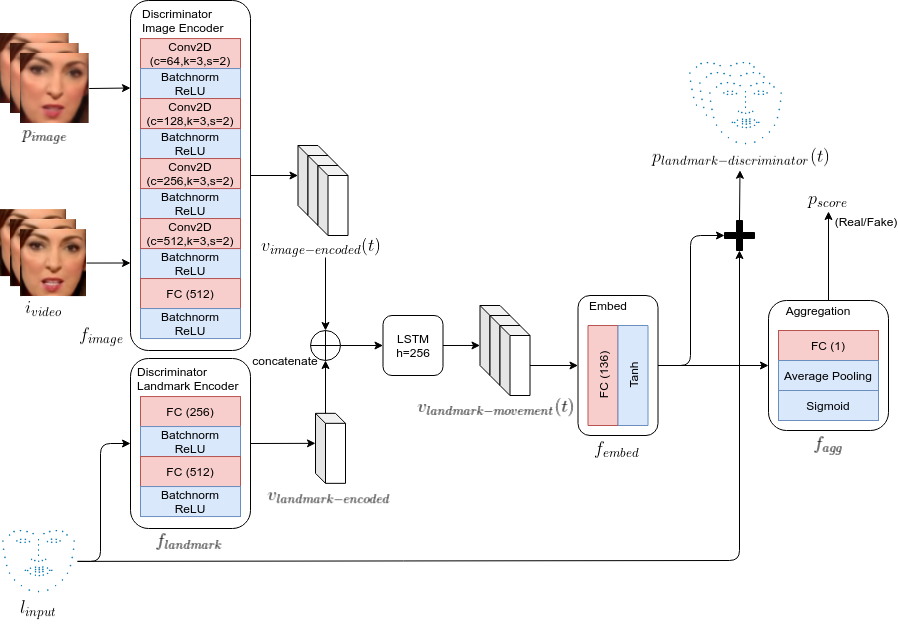
\includegraphics[width=15cm]{./content/materials/discriminator.png}
    \caption{Cấu trúc của bộ phân biệt hình ảnh (Discriminator)}
\end{figure}

\subsection{Hàm mất mát được sử dụng cho hệ Generator - Discriminator}
